\chapter{Grundlagen}
\label{ch:Grundlagen2}

Dieses Kapitel beschreibt die grundlegenden Konzepte, die für das weitere Verständnis dieser Arbeit erforderlich sind. Abschnitt \ref{sec:Decision_Management2} behandelt Decision Mangement und gibt Aufschluss darüber, wie Entscheidungen automatisiert und verwaltet werden. In Abschnitt  \ref{sec:Machine_Learning2} folgt eine Einführung in das Machine Learning. Abschließend nennt Abschnitt \ref{sec:Technologien2} einsetzbare Lösungen zur Umsetzung der genannten Konzepte. 

\section{Decision Management}
\label{sec:Decision_Management2}

\emph{Decision Management} (DM) adressiert die Verwaltung von automatisierten Entscheidungen, über den kompletten Lebenszyklus von Entscheidungen hinweg. Dieser beinhaltet die Modellierung, Ausführung, Überwachung und die Optimierung, mit dem Ziel, fachliche Entscheidungen zu verbessern, indem der Lebenszyklus kontinuierlich durchlaufen wird. Abbildung \ref{fig:lifecycle} zeigt die einzelnen Phasen des Lebenszyklus.

\begin{figure}[ht]
\centering
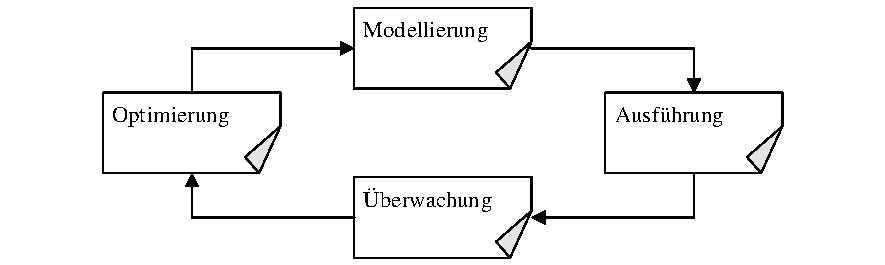
\includegraphics{images/lifecycle.pdf}
\caption{Der Lebenszyklus von automatisierten Entscheidungen.}
\label{fig:lifecycle}
\end{figure}

\textbf{Modellierung}. Zur Modellierung von Entscheidungen wurde 2015 der Standard Decison Model and Notation (DMN) von der Objekt Management Group veröffentlicht \cite[vgl. S. 7 ff.]{OM16}. Rücker nennt die Schaffung eines Notationsstandards für Entscheidungen, der für Fach- und IT-Anwender gleichermaßen verständlich ist, als übergeordnetes Ziel von DMN \cite[vgl. S. 40]{BR16}.  Die offizielle DMN-Spezifikation nennt die Erfüllung der folgenden drei Anforderungen als Ziel von DMN \cite[vgl. S. 18 ff.]{OM16}: 

\begin{enumerate*}
\item Modellierung von Entscheidungen, die von Menschen getroffen werden
\item Modellierung von Entscheidungen, die automatisiert getroffen werden 
\item Implementierung von automatisierten Entscheidungen    
\end{enumerate*}

Zur Umsetzung der genannten Anforderungen definiert DMN zwei verschiedene Ebenen: Die Entscheidungsanforderungsebene (deskriptiv) und die Entscheidungslogikebene (präskriptiv), beide zusammen bilden das \emph{Decision Model}. Auf der Entscheidungsanforderungsebene werden die Anforderungen, die eine Entscheidung benötigt, in einem Decision Requirements Diagrams (DRD) modelliert. Ein DRD besteht aus Entscheidungen, Input-Daten, Business Knowledge Models und Knowledge Sources. Abbildung \ref{fig:drd} \cite[vgl. S. 21]{OM16} zeigt die genannten Elemente eines beispielhaften DRD und deren Notation.     

\begin{figure}[ht]
\centering
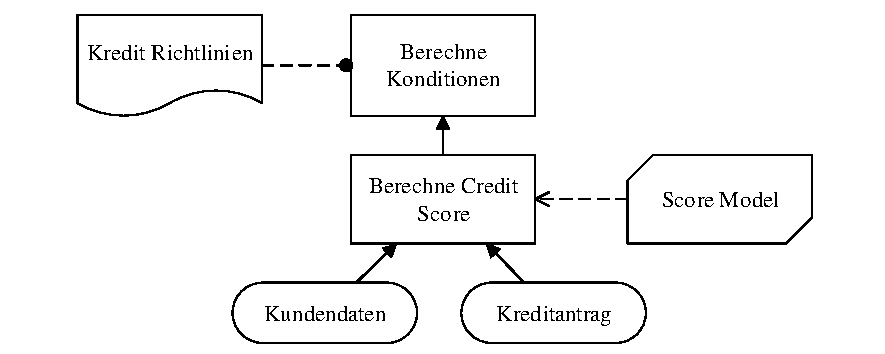
\includegraphics{images/drd.pdf}
\caption{Ein beispielhaftes DRD.}
\label{fig:drd}
\end{figure}

\begin{itemize*}

\item Ein Input-Data-Element beschreibt Informationen, die als Eingabe für eine oder mehrere Entscheidungen dient \cite[vgl. S. 30]{OM16}. Abbildung \ref{fig:drd} zeigt die beiden Input-Daten-Elemente Kundendaten und Kreditantrag. 

\item Ein Business Knowledge Model beschreibt eine Funktion die Fachwissen kapselt, beispielsweise als Geschäftsregel, Entscheidungstabelle oder als analytisches Model \cite[vgl. S. 30]{OM16}. In Abbildung \ref{fig:drd} kapselt das Score Model das Fachwissen zur Berechnung des Credit Scores.

\item Ein Decision-Element beschreibt eine Entscheidung. Sie bestimmt einen Output, anhand verschiedener Inputdaten, mithilfe von Entscheidungslogik \cite[vgl. S. 20]{OM16}. In Abbildung \ref{fig:drd} wird der Credit Score mittels der Inputdaten Kundendaten und Kreditantrag berechnet. Anschließend wird der Credit Score an die darüber liegende Entscheidung, zur Berechnung der Konditionen, weitergegeben.  

\item Eine Knowledge-Source beschreibt die Quelle einer Entscheidung oder eines Business Knowledge Models. Das kann beispielsweise ein Dokument oder auch ein Fach-Experte sein \cite[vgl. S. 18]{OM16}. Im vorliegenden Beispiel werden die Konditionen des Kredites durch die Vorgaben der Kredit Richtlinien berechnet.

\end{itemize*}

Nun gilt es sich der Entscheidungslogik-Ebene zu widmen, die insbesondere für die automatisierte Ausführung von Entscheidungen essentiell ist \cite[vgl. S. 18]{OM16}. DMN erlaubt den Import von existierenden Entscheidungslogik-Standards. Der wohl wichtigste Entscheidungslogik-Standard im Umfeld von DMN ist die Entscheidungstabelle. Taylor definiert Entscheidungstabellen als: ''a look-up table where each cell represents an executable business rule. The conditions of the rule are columns or rows in the decision table and the intersection of the rows and columns shows the consequence of the rule'' \cite[S. 132]{JT11}. Abbildung \ref{fig:decisiontable} zeigt eine Entscheidungstabelle zur Bestimmung des Zinses anhand eines Credit Scores. Wäre der Credit Score beispielsweise 632, würde die erste Zeile der Entscheidungstabelle zutreffen und der Zins 6 \%  betragen.

\begin{figure}[ht]
\centering
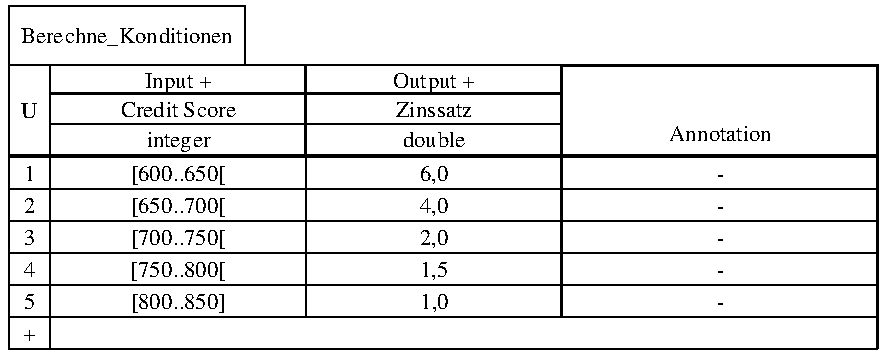
\includegraphics{images/decisiontable.pdf}
\caption{Beispiel einer Entscheidungstabelle zur Berechnung des Zinssatzes.}
\label{fig:decisiontable}
\end{figure} 

\textbf{Ausführung}. Um Decision Models ausführen zu können, müssen diese in einem geeigneten DMN-Tool modelliert werden. Zur vollständigen Automatisierung der Entscheidungen, muss die Entscheidungslogik in der Lage sein, für jeden möglichen Satz von Input-Daten einen
Entscheidungsausgang bestimmen zu können. Um eine effiziente Ausführung zu ermöglichen wird eine Decision Engine benötigt, die es erlaubt Entscheidungen in einer produktiven Einsatzumgebung auszuführen. ''Eine Decision Engine ist ein Stück Software, das eine zustandslose Schnittstelle bereitstellt, um Entscheidungen auf Basis der in DMN definierten Entscheidungslogik zu fällen'' \cite[S. 41]{BR16}. Nach der Inbetriebnahme der Decision Engine bedürfen die getroffenen Entscheidungen der Überwachung, um sicherzustellen, dass Entscheidungen so getroffen werden, dass deren Konsequenzen bestmöglich zur Erreichung der betriebswirtschaftlichen Ziele beitragen. 

\textbf{Überwachung}. Taylor nennt vier Faktoren, die kontrolliert werden sollen und dazu führen, dass Entscheidungen verbessert werden müssen \cite[vgl. S. 158]{JT11}:

\begin{enumerate*}
\item Änderungen an wirtschaftlichen Zielsetzungen
\item Neue Regularien oder Richtlinien
\item Änderungen an zugrundeliegenden Datenschemata  
\item Gesamt Performance der Entscheidungen\end{enumerate*}   

Auf die ersten drei Faktoren muss bei deren Eintritt reagiert werden, wohingegen der vierte Faktor einer ständigen Untersuchung bedarf. Proaktive Änderungen an Entscheidungslogiken bieten Möglichkeiten, die Effektivität unserer Entscheidungen zu steigern, um somit den wirtschaftlichen Zielsetzungen näher zukommen. Wie effektiv oder gut eine Entscheidung ist definiert Taylor wie folgt: ''The goals and key performance indicators or metrics of your business set a context that defines what a good or an effective decision looks like. The data you have collected over time gives you insight into what works and what doesn't, which is reflected in your current decision-making approach.'' \cite[vgl. S. 159]{JT11}. Die Analyse der Daten vergangener Entscheidungen ist somit unerlässlich, um proaktiv Entscheidungslogiken zu verbessern. Um eine effektive Überwachung und Verbesserung zu ermöglichen, müssen umfangreiche Datenmengen über die Effektivität von Entscheidungen gesammelt werden. Dazu zählen \cite[vgl. S. 164]{JT11}:

\begin{itemize*}
\item Ausführungs-Daten: Hierzu zählen alle Daten die während der Ausführung einer Entscheidung erhoben werden können. Beispielsweise IDs, Zeitstempel, Eingabe-Daten, Ausgabedaten, die Quelle des Aufrufs, oder kontextbezogene Daten die während der Ausführung generiert wurden.   
\item Antwort-Daten: Meistens ergibt sich aus einer Entscheidung heraus eine Konsequenz für den Empfänger der Entscheidung. Um nochmals das Beispiel der Online-Kredit-Bewerbung aufzugreifen, nachdem der Kreditantrag evaluiert und das Ergebnis zurückgeliefert wurde, kann die Reaktion des Empfängers gespeichert werden. Der Empfänger kann das zurückgelieferte Kreditangebot ablehnen, zustimmen, mehr Informationen verlangen oder für später abspeichern. Gelingt es die Reaktion des Empfängers mit der Entscheidung zur späteren Analyse abzuspeichern, können daraus wertvolle Rückschlüsse über die Effektivität der Entscheidung gewonnen werden.     
\item Andere Unternehmens-Daten: Neben den Daten die direkt oder indirekt durch die Entscheidung und ihre Konsequenz entstehen, macht es Sinn weitere Unternehmensdaten an vergangene Entscheidungen zuknüpfen, die später in unserer Überwachungsumgebung zu sehen sein sollen. Bei einer Entscheidung zur Berechnung der Bonität beispielsweise würde die Information, ob es zu Zahlungsausfällen kam, verknüpft mit dem entsprechenden Entscheidungsdatensatz erlauben, direkte Aussagen über die Effektivität der Entscheidungslogik zu treffen.       
\end{itemize*}         

Eine entsprechende Überwachungsumgebung müsste all diese Daten sammeln und aufbereiten, so dass der komplette Entscheidungsfindungsprozess und die daraus resultierenden Ereignisse im Nachhinein noch nachvollzogen werden können.

\textbf{Optimierung}. Um bestehende Entscheidungen optimieren zu können, bedarf es einer Simulations-Umgebung in der verschiedene Ansätze gegeneinander getestet werden können. Ein mögliches Szenario könnte so aussehen, dass man die Entscheidungslogik im Produktiveinsatz, in einem A/B Test gegen eine neue Entscheidungslogik testet. Testet man fortlaufend parallel verschiedene Ansätze kann man erkennen, welche sich langfristig am effektivsten auf wirtschaftliche Zielsetzungen auswirken \cite[vgl. S. 173]{JT11}. \emph{Predictive Analytics} eignen sich um neue Entscheidungslogiken zu entwickeln. Predictive Analytics bezeichnet \cite[vgl. S. 5]{BG15} das Verwenden von Verfahren aus der Statistik, sowie dem Machine Learning um vorherzusehen, mit welcher Wahrscheinlichkeit ein ungewisses Ereignis eintritt.   
  
\section{Machine Learning}
\label{sec:Machine_Learning2}

\emph{Machine Learning} (ML) ist eines der zentralen Themengebiete innerhalb der  \emph{Künstlichen Intelligenz} (KI) \cite[vgl. S. 2082]{JW12} und beschreibt das Forschungsgebiet das Computer befähigt zu lernen, ohne explizit dafür programmiert worden zu sein \cite[vgl. S. 1]{AM14}. Lernen im Kontext von ML definieren Mitchell et al. als: ''A computer program is said to learn from experience E with respect to some class of tasks T and performance measure P if its performance at tasks in T, as measured by P, improves with experience E'' \cite{MT97}. Soll beispielsweise ein Programm implementiert werden, das aufgrund vergangener Banktransaktionen (Experience E) lernen soll, wie man betrügerische Banktransaktionen erkennt (Task T), wird das Programm, nach erfolgreichem Lernen, besser darin sein betrügerische Banktransaktionen zu erkennen (Performance P). Der Zusammenhang zwischen Ursache und Wirkung soll mit Hilfe eines Modells beschrieben werden. Das Modell soll aus den Erfahrungen der Vergangenheit auf Ergebnisse in der Zukunft schließen können. Dabei wird versucht Eingabe- auf Ausgabewerte abzubilden, so dass die Differenz zwischen dem vorhergesagten Wert und dem realen Wert möglichst klein ist \cite[vgl. S. 68]{EM17}. Abbildung \ref{fig:lernprozess} veranschaulicht den Lernvorgang.   

\begin{figure}[ht]
\centering
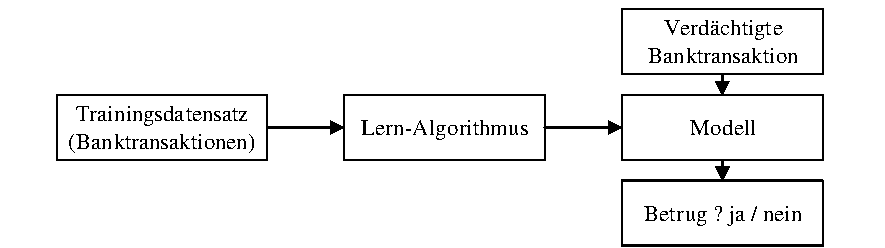
\includegraphics{images/lernprozess.pdf}
\caption{Vorgehensweise zur Entwickelung eines Modells.}
\label{fig:lernprozess}
\end{figure}  

Die Banktransaktionen, die die Trainingsdaten bilden, besitzen verschiedene Attribute, die im Kontext von ML \emph{Features} (Eingabedaten wie Alter, Geschlecht etc.) genannt werden. Neben den Attributen, die die Banktransaktion beschreiben, besitzen die Trainingsdatensätze ein \emph{Label}. Das Label bildet die Erfahrung aus der gelernt werden soll. Im vorliegenden Beispiel wäre das Label ein boolescher Wert, der angibt, ob die vorliegende Banktransaktion betrügerisch war oder nicht. Tabelle \ref{tab:trainingset} zeigt den beispielhaften Aufbau der Trainingsdaten.

\begin{table}[ht]
\centering
\small
\begin{tabular}{cccc}
\toprule
\ Feature 1 & Feature 2 & Feature 3 & Label\\
\toprule
0.86743 & 0.123 & 0.34657 & 1\\\midrule
0.26926 & 0.756 & 0.93095 & 0\\\midrule
... & ... & ... & ...\\\bottomrule
\end{tabular}
\caption{Beispielhafter Aufbau der Trainingsdaten.}
\label{tab:trainingset}
\end{table}

Abhängig von der zugrundeliegenden Problemstellung gibt es mehrere Verfahren zur Modellbildung. Zur Auswahl eines geeigneten Lern-Algorithmus, muss die Problemstellung und die vorhandenen Daten validiert und einem der folgenden Verfahren zugeordnet werden:  

\begin{itemize*}
\item \emph{Supervised-Learning}: Die Lerndatensätze bestehen aus Features und Labels. Das Modell wird trainiert, in dem man ihm vorgibt, wie Klassen richtig zugeordnet oder Werte richtig berechnet werden \cite[vgl. S. 68]{EM17}. 
\item \emph{Unsupervised-Learning}: Die Lerndatensätze besitzen keine Labels. Der Lern-Algorithmus versucht nur anhand der Inputvariablen Strukturen abzuleiten, wodurch dann das Modell gebildet wird \cite[]{SG17, EM17}. 
\item \emph{Semi-Supervised-Learning}: Eine Mischform zwischen Supervised-Learning und Unsupervised-Learning, wobei manche Trainingsdatensätze Labels besitzen können und andere nicht \cite[vgl. S. 892]{ZH10}. 
\item \emph{Reinforcement-Learning}: Das Reinforcement-Learning basiert darauf, dass ein Agent lernt, wie er sich in einer bestimmten Umgebung verhalten soll, in dem er eine Belohnung beziehungsweise eine Strafe in Form eines Skalars bekommt, der angibt wie gut oder schlecht sich der Agent verhalten hat \cite[vgl. S. 5]{WO12}.  
\end{itemize*}    

Über die Lernverfahren hinaus, müssen auch die zu berechnenden Ergebnisse der Problemstellung klassifiziert werden, um einen geeigneten Algorithmus zu finden:

\begin{itemize*}

\item \emph{Klassifikation}: Unbekannte Eingabedaten werden einer Klasse zugeordnet \cite [vgl. S. 68]{EM17}. 
\begin{itemize*}
\item Beispiel 1: Katzenfotos sollen von Hundefotos unterschieden werden.
\item Beispiel 2: Auf MRT-Bildern von Lungen soll erkannt werden, ob ein Tumor bös- oder gutartig ist.
\end{itemize*}
\item \emph{Regression}: Bestimmung eines numerischen Wertes für einen gegebenen Eingabedatensatz \cite {SG17}.   
\begin{itemize*}
\item Beispiel 1: Preisberechnung eines Gebrauchtwaagens.  
\item Beispiel 2: Vorhersage der verbleibenden Lebensdauer eines Motors.
\end{itemize*}
\item \emph{Clustering}: Beschreibt das Gruppieren von Objekten in verschiedene Gruppen. Die Datensätze einer einzelnen Untergruppe sind sich sehr ähnlich in ihren Eigenschaften, wobei die Datensätze der verschiedenen Untergruppen sehr unterschiedlich in ihren Eigenschaften sind \cite {SG17}.   
\begin{itemize*}
\item Beispiel 1: Smartphone Fotoalben, die Gesichter analysieren und Fotos nach Personen gruppieren.  
\item Beispiel 2: Analysieren von Kundendaten zur Gruppierung verschiedener Kundenklassen, für gezielte Marketingkampagnen. 
\end{itemize*}

\end{itemize*}   

Konventionelle Informationssysteme bearbeiten Aufgaben für gewöhnlich schneller als der Mensch. Nicht desto trotz handelt der Mensch in vielen Disziplinen noch ''intelligenter'' als ein Computer, als Beispiel hierfür ist die Gesichts- und Spracherkennung zu nennen. Daher liegt es nahe, dass Forscher sich am menschlichen Gehirn inspirieren lassen beim Versuch intelligente Maschinen zu entwickeln. Die Entwicklung von künstlichen neuronalen Netzen geht zurück in die 40er Jahre, als die notwendigen biologischen und elektrotechnischen Voraussetzungen vorlagen \cite [vgl. S. 1]{HS97}. Grundbaustein der menschlichen Intelligenz bilden Neuronen, die über Ein- und Ausgangsverbindungen (Synapsen) mit bis zu 200000 anderen Neuronen verbunden sein können \cite [vgl. S. 5]{SS97}. Das \textit{Perzeptron} ist ein künstliches Neuron, das in den 60er Jahren zur Mustererkennung entwickelt wurde \cite [vgl. S. 86]{EA16}. Abbildung \ref{fig:perceptron} zeigt ein Perzeptron.  

\begin{figure}[ht]
\centering

\includegraphics{images/perceptron.pdf}
\caption{Aufbau eines Perzeptrons.}
\label{fig:perceptron}
\end{figure}

Das Beispiel-Perzeptron besitzt die Inputvariablen \textit{x1}, \textit{x2}, \textit{x3}, die Gewichte \textit{w1}, \textit{w2}, \textit{w3}, sowie den Schwellenwert \textit{s}. Jede Verbindung zwischen zwei Neuronen besitzt ein Gewicht, das den Einfluss eines Neuron A auf ein Neuron B beschreibt \cite [vgl. S. 86]{EA16}. Der Ausgabewert ermittelt sich aus dem Vergleich der gewichteten Summe $\sum_j w_{j}\times x_{j}$ und einem zuvor definiertem Schwellenwert \cite {HS99, LP87, WE16}. Formel \ref{formula:perceptroneformula} \cite {HS99, WE16} zeigt den Vergleich nochmals als mathematischen Ausdruck:

\begin{align}
\label{formula:perceptroneformula}
y = \begin{cases}\text{ }0\text{ }\text{if}\text{ }\sum_j w_{j}\times x_{j}\leq s\\\text{ }1\text{ }\text{if}\text{ }\sum_j w_{j}\times x_{j}> s\end{cases}
\end{align}

Wird der Schwellenwert \textit{s} überstiegen, gibt das Perzeptron die 1 zurück anderen Falls die 0. Abbildung \ref{fig:perceptronNumbered} soll die Funktionsweise des Perzeptrons nochmals mit Hilfe von Beispiel-Werten veranschaulichen. Aus der Abbildung kann der Schwellenwert $s=6$ entnommen werden und mittels der Inputvariablen und Gewichten errechnet sich $\sum_j w_{j}\times x_{j}\text{ = 8}$. Da $\text{8}>\text{6}$ wird der Schwellenwert überstiegen und das Perzeptron liefert die 1 zurück (vgl. Formel \ref{formula:perceptroneformula}). 

\begin{figure}[ht]
\centering

\includegraphics{images/perceptronNumbered.pdf}
\caption{Modell eines Perzeptrons mit Beispiel-Daten.}
\label{fig:perceptronNumbered}
\end{figure}

Neben dem Perzeptron gibt es noch weitere künstliche Neuronen, wie z.B. das Sigmoid-Neuron. Zum Verständnis von neuronalen Netzen, ist die Betrachtung des Perzeptrons an dieser Stelle allerdings genügend. Mit einem einzigen künstlichen Neuron ist es jedoch nicht möglich, komplexere Sachverhalte abzubilden. Dies wird erst durch die Kombination vieler künstlicher Neuronen möglich. Üblicherweise besteht ein künstliches neuronales Netz aus einer Eingabe-Schicht (\emph{Input-Layer}), einer Versteckten-Schicht (\emph{Hidden-Layer}) und der Ausgabe-Schicht (\emph{Output-Layer}) \cite [vgl. S. 291]{WE16}. Abbildung \ref{fig:multilayerNN} soll diesen Sachverhalt verdeutlichen. 

\begin{figure}[ht]
\centering
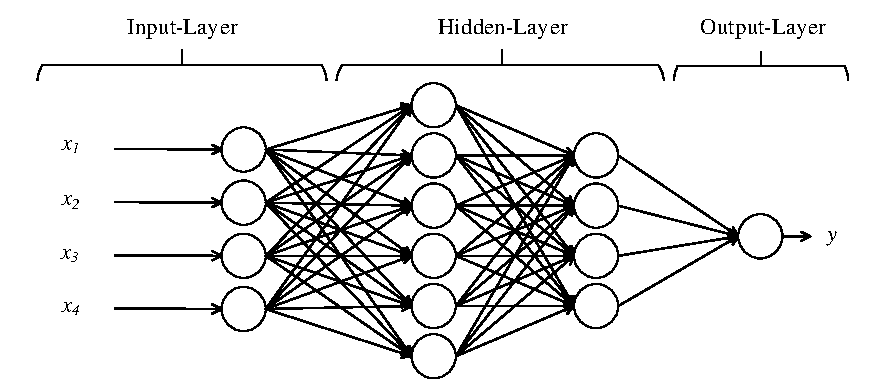
\includegraphics{images/multilayerNN.pdf}
\caption{Aufbau eines neuronalen Netzwerkes mit mehreren Schichten.}
\label{fig:multilayerNN}
\end{figure}

Dabei ist die Anzahl der Neuronen in der Hidden-Layer variabel, wohingegen die Input-Layer so viele Neuronen wie Inputvariablen besitzt. Die Anzahl der Neuronen in der Output-Layer ergibt sich durch die Anzahl der insgesamt zu berechnenden Werte des neuronalen Netzes. Soll beispielsweise ein neuronales Netz zur Erkennung von Ziffern in Bildern entwickelt werden, gäbe es zehn Neuronen in der Output-Layer, wobei jedes Neuron eine Ziffer aus dem Bereich null bis neun repräsentiert.    

Durch das Variieren der Gewichte und der Schwellenwerte, ergeben sich Modelle mit denen verschiedene Entscheidungsprozesse abgebildet werden können. Um ein Modell zu entwickeln muss das neuronale Netz lernen (trainiert werden). Im Kontext von neuronalen Netzen versteht man unter Lernen, die Modifikation der Gewichte \cite {WE16}. Zur Modifikation dieser Parameter, werden Lern-Algorithmen wie der \textit{Backpropagation-Algorithmus} verwendet. Der Backpropagation-Algorithmus wird für Supervised-Learning Problemstellungen verwendet \cite [vgl. S. 89] {EA16}, indem iterativ Datensätze durch das Neuronale-Netz gegeben werden, so dass auf Basis der Abweichung zwischen berechnetem und tatsächlichem Wert (Fehler-Funktion), die Gewichte dahingehend aktualisiert werden das die Fehler-Funktion kleiner wird.           


..................................................................
..................................................................

- Was ist Machine Learning

- Arten von Algorithmen 

- Neuronale Netze 

- Übergang: Es gibt viele verschiedene Algorithmen etc. allerdings macht es keinen Sinn mehr diese selbst zu implementieren -> Verwendung von Frameworks und somit überleiten auf nächste Kapitel

\section{Technologien}
\label{sec:Technologien2}

- Verwendung von Frameworks erforderlich um Effizient zu sein.

- Rad nicht neu erfinden evtl. Studie zur Verwendung von Frameworks.

\subsection{Decision Management}
\label{subsec:Decision_Management2}

- ACTICO 
- SAS
- FICO 
- Signavio
- Camunda

\subsection{Machine Learning}
\label{subsec:Machine_Learning2}

- Neuroph
- Aerosolve 
- Deeplearning4j
- Appache Spark

Die nachfolgende Rechnung soll das Gewicht-Update mit dem Backpropagation-Algorithmus erklären. Abbildung \ref{fig:perceptronNumberedSigmoid} zeigt ein beispielhaftes neuronales Netz mit Sigmoid-Neuronen. Ein Sigmoid-Neuron ist ein modifiziertes Perzeptron, dessen Ausgabewert jeden Wert zwischen null und eins annehmen kann. 

\begin{figure}[ht]
\centering
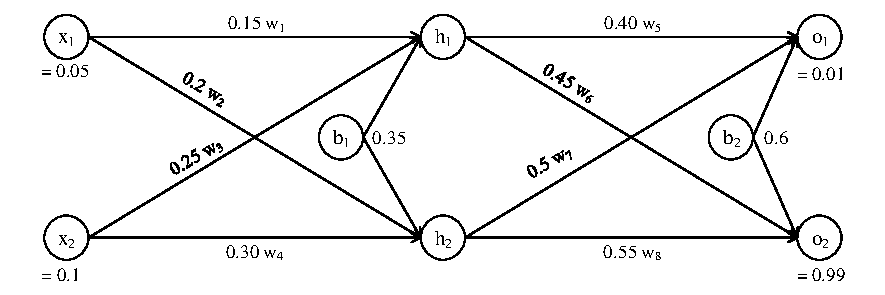
\includegraphics{images/perceptronNumberedSigmoid.pdf}
\caption{Neuronalesnetz mit Sigmoid-Neuronen und Bias.}
\label{fig:perceptronNumberedSigmoid}
\end{figure}

Das Neuronalenetz besitzt zwei Inputvariablen $x_{1}$ und $x_{2}$, zwei Outputvariablen  $o_{1}$ und $o_{2}$ und zwei Biase $b_{1}$ und $b_{2}$. Die Gewichte $w_{n}$ können den Kanten entnommen werden. Des weiteren enthält die Zeichnung den ersten Lerndatensatz. Für $x_{1} = 0,05$ und $x_{2} = 0,1$ sollen die Werte $o_{1} = 0,01$ und $o_{2} = 0,99$ vorhergesagt werden. Da das Gewicht-Update aus Basis der Fehlerrate geschieht, muss diese zuerst berechnet werden.

\begin{enumerate*}
\item Der erste Schritt beinhaltet das Berechnen der Fehlerrate mittels der Squared-Error-Funktion (siehe Formel \ref{formula:sqaurederror}). 
\begin{align}
\label{formula:sqaurederror}
E_{total} \text{ = } \sum\frac{1}{2}\textit{(target-output)}^2 
\end{align}

Dazu muss der Output $o_{1}$ für den gegeben Lerndatensatz berechnet werden, indem wir den Output des Neurons $h_{1}$ berechnen: 


$net_{h1} = w_{1} *  x_{1} + w_{2} * x_{2} + b_{1} * 1$
\\ \\
$net_{h1} = 0.15 *  0.05 + 0.2 * 0.1 + 0.35 * 1 = 0.3775$
\\ \\
Einsetzen von $net_{h1} = 0,3775$ in die Sigmoid-Funktion:
\\ \\
$out_{h1} = \frac{1}{1 + e^{-net_{h1}}} = \frac{1}{1 + e^{-0.3775}} = 0,593269992$ 

Wiederholen wir den selben Schritt für $h_{2}$ 


\item 
\begin{align}
\label{formula:chainrule}
\frac{\partial E_{total}}{\partial w} = \frac{\partial E_{total}}{\partial out} * \frac{\partial out}{\partial net} * \frac{\partial net}{\partial w}
\end{align}
\end{enumerate*} 